

\documentclass[12pt]{article}
\usepackage{graphicx}
\usepackage{amsmath}
\usepackage{mathtools}
\usepackage{gensymb}
\usepackage{tabularx}
\usepackage{array}
\usepackage[latin1]{inputenc}
\usepackage{fullpage}
\usepackage{color}
\usepackage{array}
\usepackage{longtable}
\usepackage{calc}
\usepackage{multirow}
\usepackage{hhline}
\usepackage{ifthen}
\usepackage{lscape}
\usepackage{float}
\usepackage{amssymb}

\newcommand{\mydet}[1]{\ensuremath{\begin{vmatrix}#1\end{vmatrix}}}
\providecommand{\brak}[1]{\ensuremath{\left(#1\right)}}
\providecommand{\norm}[1]{\left\lVert#1\right\rVert}
\providecommand{\abs}[1]{\left\vert#1\right\vert}
\newcommand{\solution}{\noindent \textbf{Solution: }}
\newcommand{\myvec}[1]{\ensuremath{\begin{pmatrix}#1\end{pmatrix}}}
\let\vec\mathbf

\def\inputGnumericTable{}

\begin{document}
\begin{center}
\textbf\large{OPTIMIZATION}

\end{center}
\section*{Excercise 6.6}

Q4. Find the equation of normal to the curve $x^2=4y$ which passes through the point (4,-2)

\solution
The given equation of the curve can be written as  
\begin{align}
	\label{eq:parabolaEq2}
	g\brak{\vec{x}} = \vec{x}^\top\vec{V}\vec{x} + 2\vec{u}^\top\vec{x} + f = 0 
\end{align}
where
\begin{align}
	\label{eq:eqV}
	\vec{V} &= \myvec{ 1 & 0 \\ 0 & 0} \\
	\label{eq:eqU}
	\vec{u} &= \myvec{0 \\ -2} \\
	\label{eq:eqF}
	f &= 0 
\end{align}
We are given that 
\begin{align}
	\vec{h} &= \myvec{4 \\ -2}
\end{align}
This can be formulated as optimization problem as follows:
\begin{align}
	\label{eq:Eq3}
	&  \min_{\vec{x}} \quad \text{f}\brak{\vec{x}} = \norm{\vec{x}-\vec{h}}^2\\
	\label{eq:Eq4}
	& \text{s.t.}\quad g\brak{\vec{x}} = \vec{x}^\top\vec{V}\vec{x} + 2\vec{u}^\top\vec{x} + f = 0  
\end{align}
It is already proved that the optimization problem is non-convex. We use Gradient Descent to find the optimum value. We define
\begin{align}
	\vec{x}_{n+1} = \vec{x}_n - \alpha\nabla g\brak{\vec{x}_n}
\end{align}
And the condition is given as 
\begin{align}
	\brak{\vec{x}-\vec{h}}^\top\nabla g\brak{\vec{x}_n} \neq 0
\end{align}
Now we choose the parameters as
\begin{enumerate}
	\item $\alpha$ = 0.001
	\item precision = 0.001
	\item n = 10000
	\item $\vec{x}_0$ = 4
\end{enumerate}
We get the minimum value of $\vec{x}$ as
\begin{align}
	\vec{x}_{min} = \myvec{1.695\\0.718}
\end{align}
See figure \ref{fig:Fig1}
\begin{figure}[!h]
	\begin{center} 
	    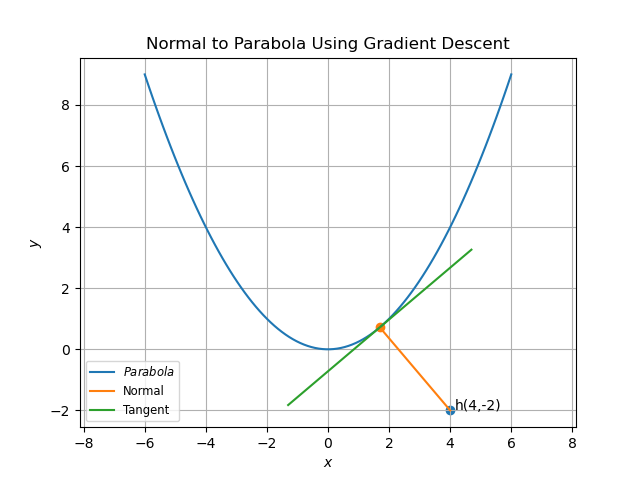
\includegraphics[width=\columnwidth]{figs/12_6_6_4_gradient}
	\end{center}
\caption{}
\label{fig:Fig1}
\end{figure}
\end{document}

































